\documentclass[12pt,letterpaper]{article}
\usepackage{listings}
\usepackage{graphicx}
\usepackage[table,xcdraw]{xcolor}
\RequirePackage{xcolor}
\definecolor{tecAzul}{cmyk}{1,0.91,0.33,0.25} % según manual de imagen 2016
\definecolor{tecRojo}{cmyk}{0,0.9,0.86,0}     % según manual de imagen 2016

\renewcommand{\familydefault}{\sfdefault}
\usepackage{amsmath} % for the equation* environment
\usepackage{mwe}
\usepackage{graphicx}
\usepackage[spanish]{babel}
\usepackage{multirow}
\usepackage{titlesec}
\titleformat*{\section}%
{\normalfont\Large\bfseries\color{tecAzul}}
\titleformat*{\subsection}%
{\normalfont\large\bfseries\color{tecAzul}}


\usepackage[tmargin=2cm,bmargin=2cm,lmargin=2.5cm,rmargin=2.5cm]{geometry}
\usepackage{textpos}
\usepackage{tikz}
\usepackage{pgfplots}
\usepackage{pgf}

\usepackage[margin=1cm]{caption}

\usepackage{hyperref}

%
% paragraph layout
%
\parindent0em                           % indentation width of first line
\parskip1.3ex                           % space between paragraphs


\newcommand{\EstudianteA}{David F. Duarte Sánchez}

\pgfplotsset{compat=1.17}



\usepackage{listings}
\usepackage{xcolor}

\definecolor{codegreen}{rgb}{0,0.6,0}
\definecolor{codegray}{rgb}{0.5,0.5,0.5}
\definecolor{codepurple}{rgb}{0.58,0,0.82}
\definecolor{backcolour}{rgb}{0.95,0.95,0.92}

\lstdefinestyle{mystyle}{
    backgroundcolor=\color{backcolour},   
    commentstyle=\color{codegreen},
    keywordstyle=\color{magenta},
    numberstyle=\tiny\color{codegray},
    stringstyle=\color{codepurple},
    basicstyle=\ttfamily\footnotesize,
    breakatwhitespace=false,         
    breaklines=true,                 
    captionpos=b,                    
    keepspaces=true,                 
    numbers=left,                    
    numbersep=5pt,                  
    showspaces=false,                
    showstringspaces=false,
    showtabs=false,                  
    tabsize=2
}

\lstset{style=mystyle}



\begin{document}
	
\graphicspath{{./}{./fig/}}

%-------------------------- Title section -------------------------------------%

%
\begin{textblock}{10}[0,0](-0.5,0)
	\large Escuela de Ingeniería Electrónica \\ 
	EL5617 Trabajo Final de Graduación \\
\end{textblock}

%
\begin{textblock}{10}[0,0](2.6,-0.35)
	\begin{flushright}
		
\includegraphics[scale=0.8]{Firma_TEC-4.pdf}
	\end{flushright}
\end{textblock}

%% Title %%
\begin{center}
	\vspace{70mm}
	{\large\color{tecRojo} Trabajo Final de Graduación}
	\par\vspace{8mm}
	{\Large\bf\color{tecAzul}{Bitácora de Trabajo - Entrega 3}}
	\par\vspace{100mm}
	{{\EstudianteA \\ II Semestre 2024} 
	\vspace{8mm}}
\end{center}

\newpage
%------------------------------------------------------------------------------%

\renewcommand{\baselinestretch}{1.1}    % line spacing

%------------------------------------------------------------------------------%

\section{Semana 8}
\subsection{Corrección de Tesis}

\bf{Fecha de trabajo:} 06/09/2024.\\
\bf{Objetivo:} Corrección de observaciones realizadas a la Tesis.

\begin{table}[h!]
    \resizebox{\textwidth}{!}{%
    \begin{tabular}{|l|}
        \hline
        \hline
        \multicolumn{1}{|c|}{Reporte de   actividades} \\ \hline
        \hline
        -Se comienza a elaborar la sección 1 y 3 de la Tesis con el fin de revisar el estado final \\
        de estos en la próxima reunión programada para control de las tesis, además de esto se\\
        puede comenzar a realizar el primer capítulo de la Tesis, ya que el comité ha aprobado el \\
        anteproyecto. \\ \hline
        
        - Se comienza la elaboración de un manual de usuario, con el fin de hacer más fácil la \\
        evaluación del flujo de trabajo y la depuración del mismo, de esta forma se tendrán\\
        estandarizadas las versiones requeridas y las salidas esperadas en cada uno de los \\
        procedimientos que se realizan a lo largo de la experimentación. \\ \hline
        
        - Exploración sobre mejores versiones de Ubuntu sobre la cual se puedan trabajar los contenedores\\
        primeramente se creía que un contenedor de Ubuntu 18.04 era la mejor aproximación, pero se ha encontrado\\
        que la versión 16.04 es más estable y permite un mejor desarrollo del flujo de trabajo\\ \hline

        - Generación de un archivo Docker con el fin de generar una receta para montar más sencillamente soluciones\\
        en el ambiente propuesto de trabajo, de esta forma se estandarizan las versiones requeridas, evitando de esta \\
        forma futuros problemas de versión los cuales son muy delicados cuando se trata con ambientes embebidos. \\ \hline\hline

        \hline
        \multicolumn{1}{|c|}{Productos obtenidos} \\ \hline\hline
        Se comienza la elaboración del capítulo 1 y 3 además de la finalización del capítulo\\
        2 esto con el fin de buscar referencias bibliográficas de utilidad a la hora de\\
        poder implementar los pasos descubiertos en este periodo de investigación, seguido\\
        de esto se comienza con la elaboración de un manual de usuario el cual sea de utilidad\\
        a la hora de replicar el sistema realizado.\\

        Al trabajar con Ubuntu y Yocto, las versiones de los requerimientos son fundamentales,\\
        ya que de estas depende la correcta implementación del flujo de trabajo, al hacer \\
        referencia a esto se tenían dos panoramas, en el primero de ellos trabajamos con un \\
        ambiente virtual, pero este mostraría limitantes a la hora de tratar de exportarlo\\
        y llevarlo al siguiente paso. Es por esto que se utiliza un contenedor en Docker donde\\
        se genera con la versión de Ubuntu requerida mediante un archivo de generación.\\
        
        Es así como se logra determinar que la versión 16.04 es más estable que la 18.04 para\\
        la elaboración del flujo de trabajo.\\ \hline \hline  
    \end{tabular}}
\end{table}

Como se mencionó anteriormente se logró encontrar un BSP disponible para la ZeadBoard, el mismo
se encuentra actualmente disponible para la distribución de Yocto Zeus la cual tuvo el lanzamiento 
en el año de 2019, por tanto es necesario instalar Ubuntu 18.04 para poder llevar a cabo la elaboración
del conjunto de flujos de trabajo. Los mismos se realizan siguiendo esta serie de pasos. 

Tabla con las versiones de Yocto

\begin{table}[h!]
    \caption{}
    \label{tab:my-table}
    \resizebox{\textwidth}{!}{%
    \begin{tabular}{|l|l|l|l|l|l|l|}
    \hline
    \rowcolor[HTML]{EAECF0} 
    \multicolumn{1}{|c|}{\cellcolor[HTML]{EAECF0}{\color[HTML]{202122} \textbf{Codename}}} &
      \multicolumn{1}{c|}{\cellcolor[HTML]{EAECF0}{\color[HTML]{202122} \textbf{Yocto Project Version}}} &
      \multicolumn{1}{c|}{\cellcolor[HTML]{EAECF0}{\color[HTML]{202122} \textbf{Release Date}}} &
      \multicolumn{1}{c|}{\cellcolor[HTML]{EAECF0}{\color[HTML]{202122} \textbf{Current Version}}} &
      \multicolumn{1}{c|}{\cellcolor[HTML]{EAECF0}{\color[HTML]{202122} \textbf{Support Level}}} &
      \multicolumn{1}{c|}{\cellcolor[HTML]{EAECF0}{\color[HTML]{202122} \textbf{Poky Version}}} &
      \multicolumn{1}{c|}{\cellcolor[HTML]{EAECF0}{\color[HTML]{202122} \textbf{BitBake branch}}} \\ \hline
    \rowcolor[HTML]{F8F9FA} 
    {\color[HTML]{708090} Zeus} &
      {\color[HTML]{708090} 3.0} &
      {\color[HTML]{708090} October 2019} &
      {\color[HTML]{708090} 3.0.4 (August 2020)} &
      {\color[HTML]{708090} EOL} &
      {\color[HTML]{708090} 22.0.3} &
      {\color[HTML]{708090} 1.44} \\ \hline
    \rowcolor[HTML]{F8F9FA} 
    {\color[HTML]{708090} Dunfell} &
      {\color[HTML]{708090} 3.1} &
      {\color[HTML]{708090} April 2020} &
      {\color[HTML]{708090} 3.1.33 (May 2024)} &
      {\color[HTML]{708090} EOL - LTS¹} &
      {\color[HTML]{708090} 23.0} &
      {\color[HTML]{708090} 1.46} \\ \hline
    \end{tabular}%
    }
    \end{table}

Tabla con las versiones de paquete de soporte de tarjeta según el repo de Xilinx

Indicar que se sigue bajo la investigación si hay alguna versión LTS que soporte el ZedBoard
- Se logra encontrar que la versión 16.04 LTS puede ejecutar el flujo de trabajo requerido para la correcta generación del 
flujo de trabajo

Primeramente se genera el ambiente de trabajo.
\begin{lstlisting}[language=bash]
  docker pull ubuntu:16.04
  docker run -it ubuntu:16.04
\end{lstlisting}

Con las instrucciones mostradas anteriormente se genera un contenedor con la versión de Ubuntu 16.04.

Seguido de esto se debe de generar un usuario no root, esto con el objetivo de no generar alarmas más adelante
en la generación de la imagen embebida

\begin{lstlisting}[language=bash]
  # Update package lists
  apt-get update
  
  # Install sudo if it's not already installed
  apt-get install -y sudo
  
  # Create a new user with a home directory
  useradd -ms /bin/bash myuser
  
  # Set a password for the new user
  echo "myuser:password" | chpasswd
  
  # Add the new user to the sudo group
  usermod -aG sudo myuser
  
  
  su - myuser
\end{lstlisting}

Una vez generado el usuario no root y registrado en el mismo se deben de seguir estos pasos:

\begin{lstlisting}[language=bash]
  apt-get update
  apt-get install -y locales
  
  locale-gen en_US.UTF-8
  
  dpkg-reconfigure locales
  
  locale
  
  export LANG=en_US.UTF-8
  export LC_ALL=en_US.UTF-8
  
  locale
\end{lstlisting}

Este paso se realiza para que Python sepa interpretar correctamente los caracteres contenidos en el formato mencionado
anteriormente.
Una vez concluidos estos pasos se puede continuar con la parte existente del instructivo 

\begin{lstlisting}[language=bash]
sudo apt-get install gawk wget git-core diffstat unzip texinfo 
gcc-multilib build-essential chrpath socat cpio python python3 
python3-pip python3-pexpect xz-utils debianutils iputils-ping 
python3-git python3-jinja2 libegl1-mesa libsdl1.2-dev pylint3
xterm

git clone -b zeus https://git.yoctoproject.org/git/poky
cd poky

git clone -b zeus https://github.com/Xilinx/meta-xilinx
git clone -b zeus https://github.com/openembedded/meta-openembedded.git

source oe-init-build-env

echo "MACHINE??=\"zedboard-zynq7\"" >> conf/local.conf
echo "IMAGE_FEATURES += \"package-management\"" >> conf/local.conf
echo "DISTRO_HOSTNAME = \"zynq\"" >> conf/local.conf

bitbake-layers add-layer ../meta-xilinx/meta-xilinx-bsp/
bitbake-layers add-layer ../meta-openembedded/meta-oe/

bitbake core-image-minimal
\end{lstlisting}

\begin{figure}[h!]
    \centering
    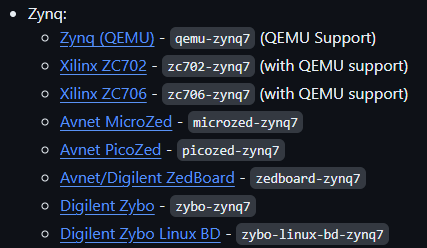
\includegraphics[width=0.8\textwidth]{images/image01.png}
    \caption{BSP Xilinx}
    \label{fig:Entorno}
  \end{figure}

%\bibliography{bibliografia_consultada}
%\bibliographystyle{plain}
\end{document}